% Kapitel 1 Arbeitsgrundlagen------------------------------------------------- %
\section{Arbeitsgrundlagen}
% ---------------------------------------------------------------------------- %
In diesem Abschnitt werden die Arbeitsgrundlagen zur Beugung und Interferenz für den Versuch erarbeitet.
% **************************************************************************** %
\subsection{Beugung}
% **************************************************************************** %


% **************************************************************************** %
\subsection{Interferenz}
% **************************************************************************** %

\subsubsection{Frauenhofer'sche Beobachtungsart}
Bei der Frauenhofer'sche Beobachtungsart wird das Interfernzmuster, wie in der Abbildung \ref{fig:beobachtungsart} dargestellt, in der Brennebene beobachtet. Dies geschieht in dem das Interferenzmuster durch eine Linse auf einen Schirm projiziert wird. Die Linse wird im Abstand $ f $ vor dem Schirm platziert. Das beobachtete Muster ist bis auf einen Skalierungsfaktor identisch zum Interferenzmuster, welches in grosser Entfernung von den Quellen beobachtet werden kann. Der Abstand von der Linse von den Quellen hat keinen Einfluss auf die Abmessung oder die Form des Interferenzmuster. Er bestimmt nur den erfassten Winkelbereich.

\begin{figure}[h!]
	\centering
	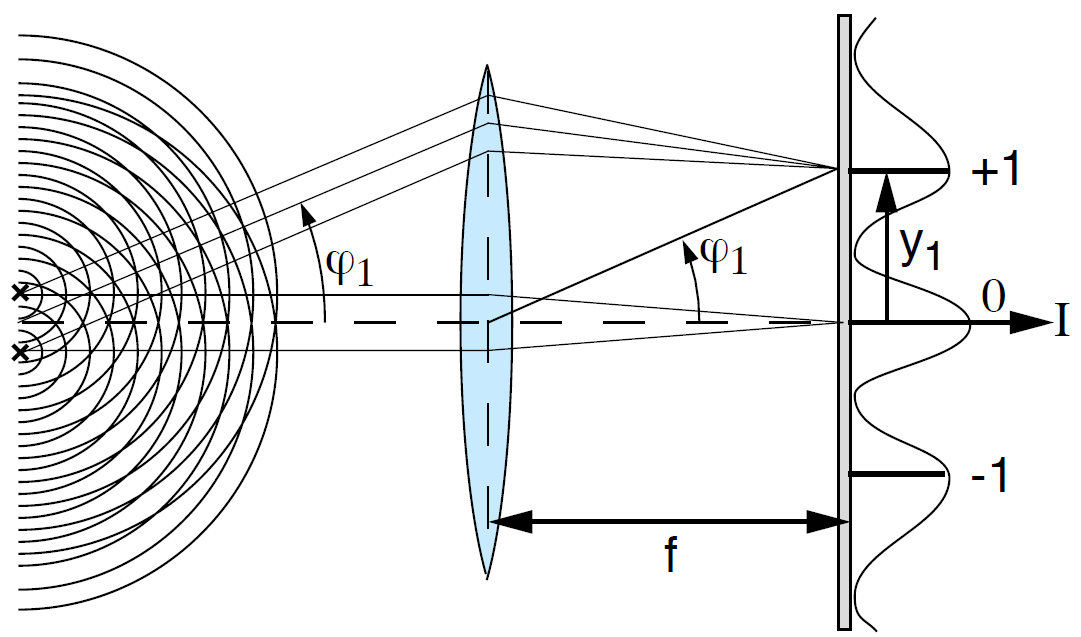
\includegraphics[width=0.8\textwidth]{data/fraunhofer}
	\caption{Frauenhofer'sche Beobachtungsart}
	\label{fig:beobachtungsart}
\end{figure}

Der Winkel $ \phi_{1} $ der Interferenz erster Ordnung kann mit dem Abstand $ y_{1} $ von dem Hauptstrahl zum Extrema der ersten Ordnung und der Brennweite $ f $ der Linse wie folgt berechnen.
\begin{equation}\label{eq:frauenhofer}
tan(\phi_{1}) =  \frac{y_{1}}{f}
\end{equation}

\subsubsection{Beugung am Spalt und Antispalt}

\begin{figure}[h!]
	\centering
	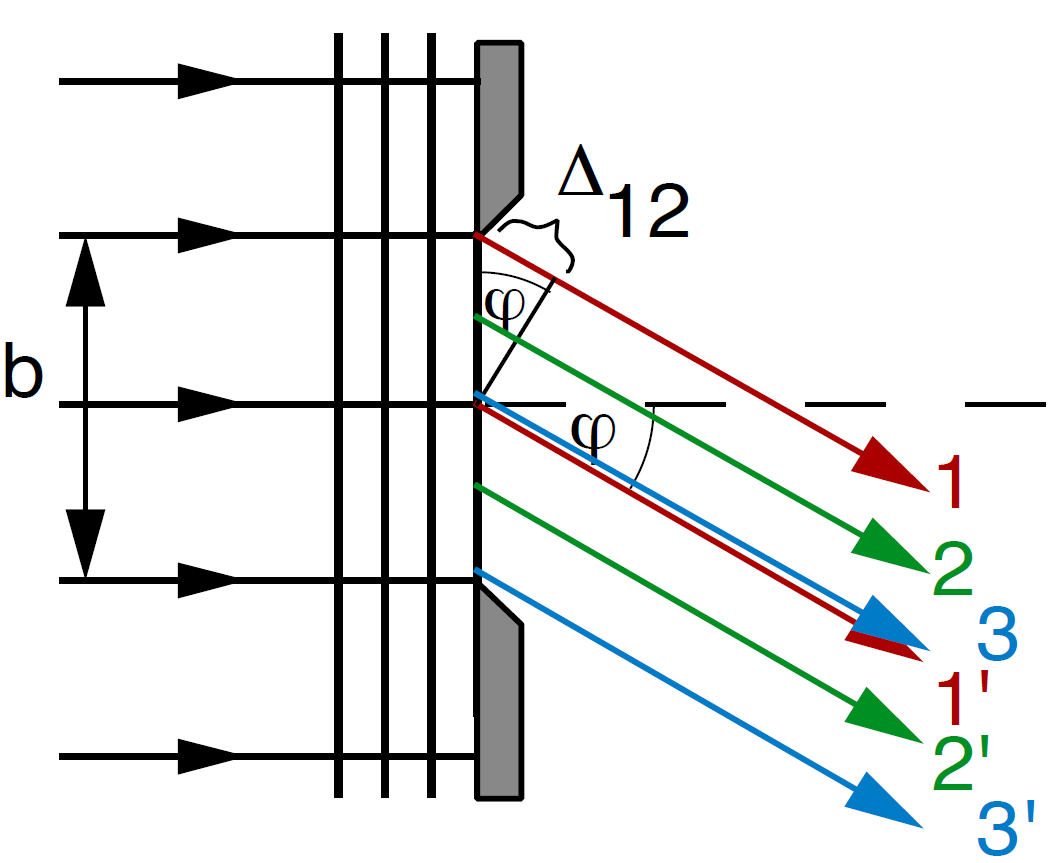
\includegraphics[width=0.4\textwidth]{data/spalt}
	\caption{Beugung an einem Spalt}
	\label{fig:spalt}
\end{figure}

\subsubsection{Beugung am Loch und Antiloch}

\begin{figure}[h!]
	\centering
	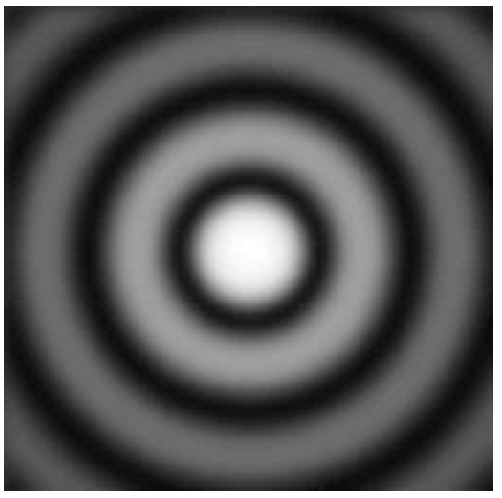
\includegraphics[width=0.3\textwidth]{data/loch}
	\caption{Interferenzmuster einer Beugung an einem Loch}
	\label{fig:loch}
\end{figure}

\subsubsection{Beugung am Strichgitter}

\begin{figure}[h!]
	\centering
	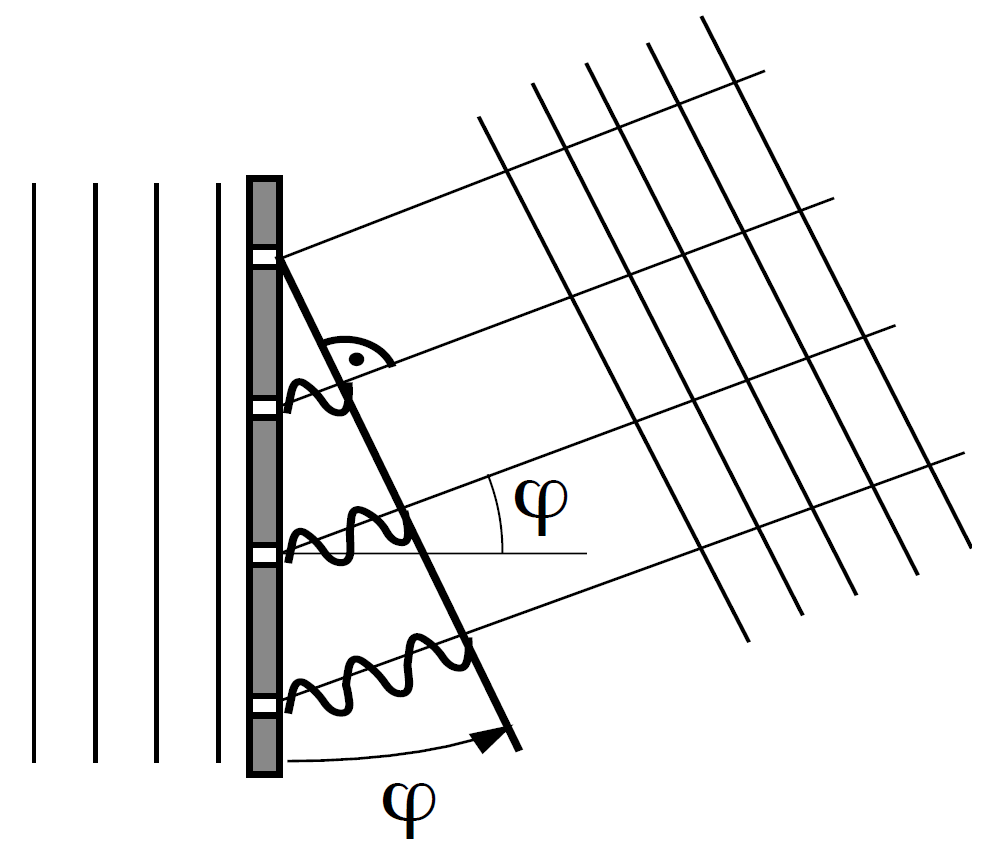
\includegraphics[width=0.4\textwidth]{data/gitter}
	\caption{Beugung an einem Strichgitter}
	\label{fig:gitter}
\end{figure}


